\documentclass[border=6pt]{standalone}
\usepackage{times}
\usepackage{pgfplots}
\pgfplotsset{compat=1.18}
\begin{document}
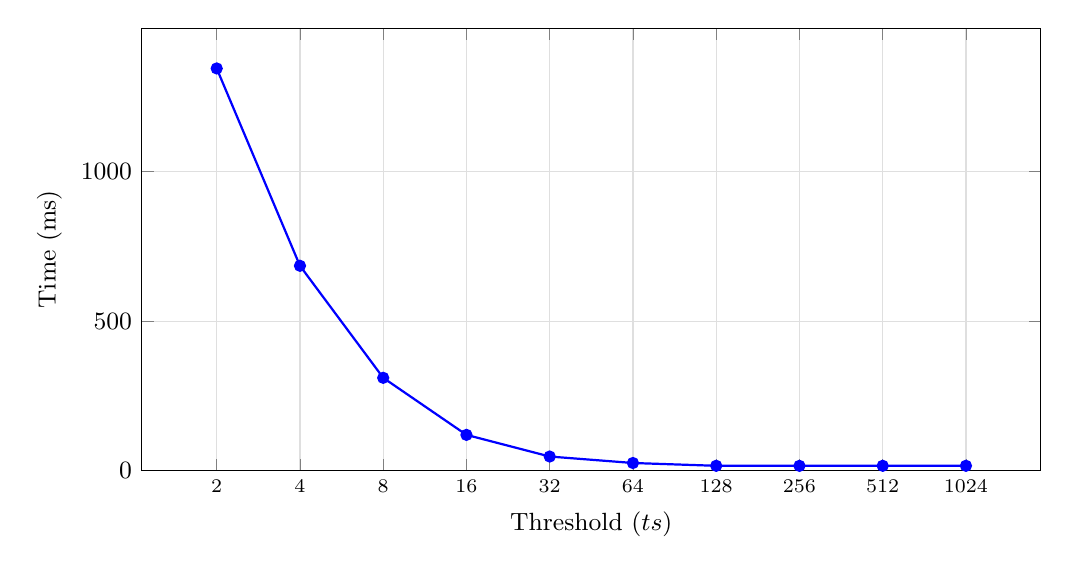
\begin{tikzpicture}
\begin{axis}[width=13cm,height=7.2cm,
xlabel={Threshold ($ts$)},ylabel={Time (ms)},
xmode=log,log basis x=2,xtick={2,4,8,16,32,64,128,256,512,1024},xticklabels={2,4,8,16,32,64,128,256,512,1024},x tick label style={font=\scriptsize},
ymin=0,grid=both,major grid style={gray!25},minor grid style={gray!10},
tick label style={font=\small},label style={font=\small},
scaled y ticks=false,/pgf/number format/1000 sep={}]
\addplot[blue,thick,mark=*,mark size=1.8pt] coordinates {
(2, 1345.547635)
(4, 685.272607)
(8, 310.478245)
(16, 119.603401)
(32, 47.15816)
(64, 25.506483)
(128, 16.135097)
(256, 15.926473)
(512, 16.072596)
(1024, 16.124346)
};
\end{axis}
\end{tikzpicture}
\end{document}
